\documentclass[a4 paper, 15pt]{article}
% Set target color model to RGB
\usepackage[inner=2.0cm,outer=2.0cm,top=2.5cm,bottom=2.5cm]{geometry}
\usepackage{setspace}
\usepackage[rgb]{xcolor}
\usepackage{verbatim}
\usepackage{subcaption}
\usepackage{amsgen,amsmath,amstext,amsbsy,amsopn,tikz,amssymb,tkz-linknodes}
\usepackage{fancyhdr, float}
\usepackage[colorlinks=true, urlcolor=blue,  linkcolor=blue, citecolor=blue]{hyperref}
\usepackage[colorinlistoftodos]{todonotes}
\usepackage{rotating,listings}
%\usetikzlibrary{through,backgrounds}
%\usetikzlibrary{shadows}
\usepackage{booktabs}
\newcommand{\ra}[1]{\renewcommand{\arraystretch}{#1}}


\lstset{language=Python,
        basicstyle=\ttfamily\small,
        keywordstyle=\color{keywords},
        commentstyle=\color{comments},
        stringstyle=\color{red},
        showstringspaces=false,
        identifierstyle=\color{green},
        procnamekeys={def,class}}

\newtheorem{thm}{Theorem}[section]
\newtheorem{prop}[thm]{Proposition}
\newtheorem{lem}[thm]{Lemma}
\newtheorem{cor}[thm]{Corollary}
\newtheorem{defn}[thm]{Definition}
\newtheorem{rem}[thm]{Remark}
\numberwithin{equation}{section}

\newcommand{\homework}[6]{
   \pagestyle{myheadings}
   \thispagestyle{plain}
   \newpage
   \setcounter{page}{1}
   \noindent
   \begin{center}
   \framebox{
      \vbox{\vspace{2mm}
    \hbox to 6.28in { {\bf CS 6780:~Advanced Machine Learning \hfill {\small (#2)}} }
       \vspace{6mm}
       \hbox to 6.28in { {\Large \hfill #1  \hfill} }
       \vspace{6mm}
       \hbox to 6.28in { {\it Instructor: {\rm #3} \hfill Name: {\rm #5}, Netid: {\rm #6}} }
       %\hbox to 6.28in { {\it TA: #4  \hfill #6}}
      \vspace{2mm}}
   }
   \end{center}
   \markboth{#5 -- #1}{#5 -- #1}
   \vspace*{4mm}
}
\newcommand{\problem}[2]{~\\\fbox{\textbf{Problem #1}}\hfill (#2 points)\newline\newline}
\newcommand{\subproblem}[1]{~\newline\textbf{(#1)}}
\newcommand{\D}{\mathcal{D}}
\newcommand{\Hy}{\mathcal{H}}
\newcommand{\VS}{\textrm{VS}}
\newcommand{\solution}{~\newline\textbf{\textit{(Solution)}} }


\begin{document}
\homework{Submission Assignment \#1}{Due: 02/12/19}{Thorsten Joachims}{}{Molly Ingram, Julien Neves}{msi34, jmn252}
\textbf{Course Policy}: Read all the instructions below carefully before you start working on the assignment, and before you make a submission.
\begin{itemize}
    \item Please typeset your submissions in \LaTeX. Use the template provided in {\tt a1\_template.tex} for your answers. Please include your name and NetIDs with submission.
date and time on the first page.
    \item Assignments are due at the beginning of class at 2:55 pm on the due date on CMS.
    \item Late assignments can be submitted on CMS up to Sunday, Feb 17. This is also when the solutions will be released.
    \item You can do this assignment in groups of 2. Please submit no more than one submission per group.
    \item All sources of material must be cited. The University Academic Code of Conduct
will be strictly enforced.
\end{itemize}

\problem{1: Version Spaces}{5+5+5+10=25}
\begin{table}[h]
\centering
\begin{tabular}{@{}lll|l@{}}
\toprule
\textit{Weather} & \textit{Food} & \textit{Meeting} & \textit{Attend?} \\ \midrule
cold             & full          & idc              & yes              \\
cold             & empty         & no               & no               \\
hot              & full          & yes              & yes              \\
cold             & full          & no               & yes              \\
hot              & empty         & no               & no               \\ \bottomrule
\end{tabular}
\caption{Dataset $\D$\label{table:1}}
\end{table}


\subproblem{a}
\begin{table}[h]
\centering
\begin{tabular}{@{}lll|l@{}|llll}
	\toprule
	\textit{Weather} & \textit{Food} & \textit{Meeting} & \textit{Attend?} & $h_{A}$ & $h_{B}$ & $h_{C}$ & $h_{D}$  \\ \midrule
	cold             & full          & idc              & yes             & y & y & y & n  \\
	cold             & empty         & no               & no              & y & n & n & n  \\
	hot              & full          & yes              & yes             & y & y & y & n  \\
	cold             & full          & no               & yes             & y & y & y & y  \\
	hot              & empty         & no               & no              & y & n & n & n  \\ \bottomrule
\end{tabular}
\caption{Dataset $\D$ with Predictions\label{table:2}}
\end{table}

\subproblem{b} As we can see from Table 2, only $h_{B}$ and $h_{C}$ are in $\VS(\D)$ because they are the only consistent hypotheses.

\subproblem{c} With the new data point, only $h_{B}$ is consistent so only $h_{B}$ is in $\VS(\D)$.

\subproblem{d}

I have modified the notation of the problem for clarity. I am specifying that each  $x_{i} \in \{0, 1\}^{k+1}$, so there are $k$ attributes and one output to predict. If I had $2^{k}$ data points and only $k-1$ attributes, I could not create a consistent decision tree.  For example, the dataset $(X,Y) = \{(1,0),(0,1),(1,1),(0,0)\}$ does not have a consistent decision tree.

Let $k \in \mathbb{Z}_{+}$. Consider a dataset $\D = \{x_{1}, x_{2}, . . . , x_{2^{k}}\}$ such that $x_{i} \in \{0, 1\}^{k+1}$ and $x_{i} \ne x_{j} \forall i\ne j$ . Let $X$ be the first $k$ attributes of each datapoint and $Y$, the remaining attribute, be the output variable to predict. Consider a decision tree where the first decision node is (Attribute 1 == value), the second decision node is (Attribute 2 == value), and so on where the $k^{th}$ decision node is (Attribute $k$ == value). Since each attribute is binary, the tree ends with $2^{k}$ leaf nodes.  Because $x_{i} \ne x_{j} \forall i\ne j$, each path down the tree corresponds to one datapoint, thus the decision tree is consistent and an element of $\VS(\D)$.

\newpage
\problem{2: Decision Trees, Overfitting}{5+10+10+5+10+10=50}

\subproblem{a}

Table \ref{table:3} reports the count for the diagnosis labels of the training set.
\begin{table}[h]
\centering
\begin{tabular}{l|l}
	\toprule
	\textit{Label} & \textit{Count} \\ \midrule
1 & 484 \\
0 & 416
   \bottomrule
\end{tabular}
\caption{Dataset $\D$ with Predictions\label{table:3}}
\end{table}

While split pretty evenly, the majority label is $1$. Therefore, if use $1$ as our predition for every case we get the accuracy scores reported in Table \ref{table:4}.

\begin{table}[h]
\centering
\begin{tabular}{l|l}
	\toprule
	\textit{Set} & \textit{Accuracy score} \\ \midrule
Training & 53.78\% \\
Test & 50.60\%
   \bottomrule
\end{tabular}
\caption{Accuracy scores for baseline model\label{table:4}}
\end{table}

\subproblem{b}

Table \ref{table:5} reports the accuracy scores for the implementation of the decision tree with default parameters.
\begin{table}[h]
\centering
\begin{tabular}{l|l}
	\toprule
	\textit{Set} & \textit{Accuracy score} \\ \midrule
Training & 100\% \\
Test & 56.18\%
   \bottomrule
\end{tabular}
\caption{Accuracy scores for decision tree\label{table:5}}
\end{table}

As we can see, we get perfect prediction on the training set while only slightly better prediction accuracy, i.e. $56.18\%>50.60\%$.

While we get a accuracy of 100\% on the training, this might not be the optimal model has we might be overfitting our training set which could yield poor predictive power. This is the classic trade-off between variance and bias.

\subproblem{c}

Looking at the attributes of our fitted \texttt{DecisionTreeClassifier}, we have a \texttt{max\_depth} of $21$.

Figure \ref{fig:1} show the accuracy scores for different values of \texttt{max\_depth}.

\begin{figure}[H]
  \centering
  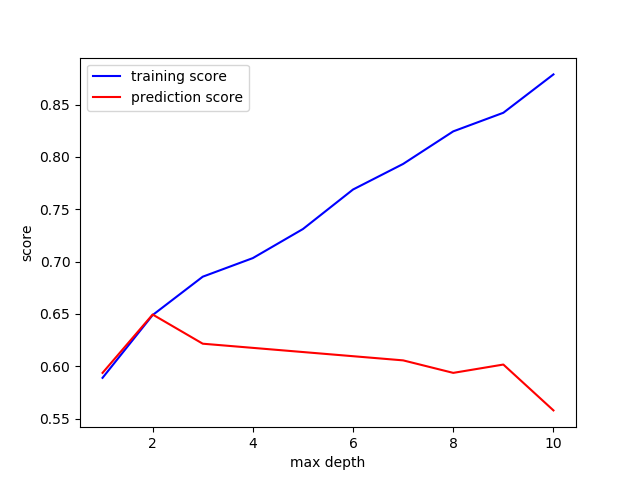
\includegraphics[width=0.5\textwidth]{fig_1}
  \caption{Accuracy scores for decision tree\label{fig:1}}
\end{figure}

As we can see, while the accuracy score on the training increases steadily as \texttt{max\_depth} increases, the prediction score increase up to \texttt{max\_depth}=2 and then starts decreasing. This indicates that we might be better off with a simpler model than one with \texttt{max\_depth}=21.


\subproblem{d}

Akin to p-hacking, if we play around with the parameters enough, we will find a spurious model that will seem to be able to predict the data perfectely solely for this peculiar context. For robustness, it is better to have a simpler model.

\subproblem{e}

Figure \ref{fig:2} show the accuracy scores for the 4-fold cross-validation for different values of \texttt{max\_depth}.

\begin{figure}[H]
  \centering
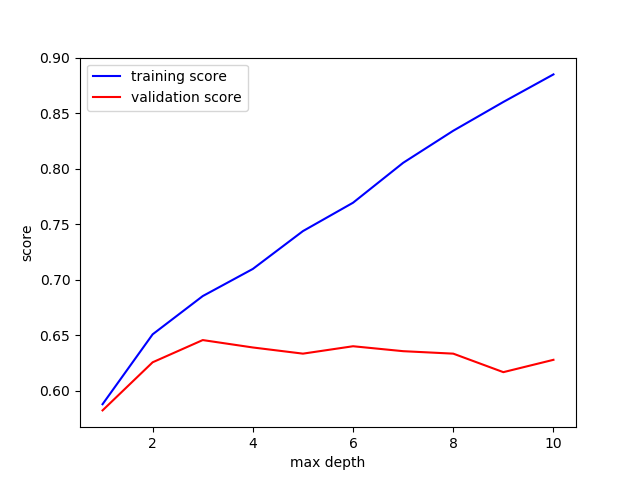
\includegraphics[width=0.5\textwidth]{fig_2}
  \caption{4-fold validation curves\label{fig:2}}
\end{figure}

The depth that gives us the best perfomance is 3. We therefore use \texttt{max\_depth}=3 and report the accuracy scores on the whole training set and test set in Table \ref{table:6}.

\begin{table}[h]
\centering
\begin{tabular}{l|l}
	\toprule
	\textit{Set} & \textit{Accuracy score} \\ \midrule
Training & 68.56\% \\
Test & 62.15\%
   \bottomrule
\end{tabular}
\caption{Accuracy scores with \texttt{max\_depth} = 3 \label{table:6}}
\end{table}



\subproblem{f}

Figure \ref{fig:3} show the accuracy score for the 4-fold cross-validation for different number of k-best features and \texttt{max\_depth} = 10.

\begin{figure}[H]
  \centering
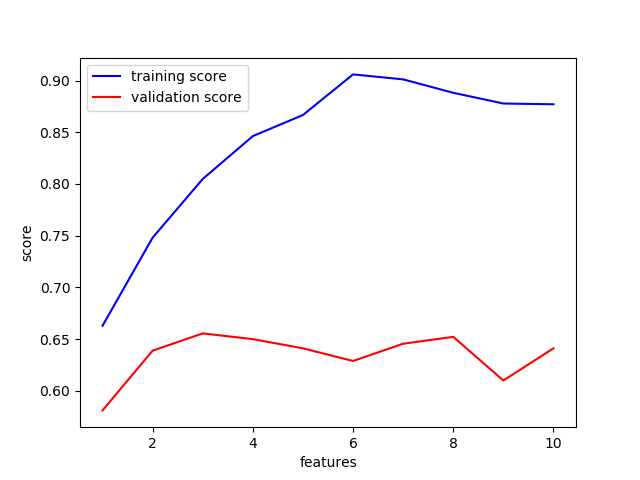
\includegraphics[width=0.5\textwidth]{fig_3}
  \caption{4-fold validation curves with \texttt{max\_depth} = 10\label{fig:3}}
\end{figure}

It is not clear from just the graph but it seems like the best number of k-best features is 3.

Table \ref{table:7} reports the accuracy score for using the first 3-best features and a maximum depth of 10.

\begin{table}[h]
\centering
\begin{tabular}{l|l}
	\toprule
	\textit{Set} & \textit{Accuracy scores} \\ \midrule
Training & 79.67\% \\
Test & 68.13\%
   \bottomrule
\end{tabular}
\caption{Accuracy score with \texttt{max\_depth} = 10 and 3-best features\label{table:7}}
\end{table}

Therefore, this simpler decision tree seems to outperform every single model we considered so far.


\newpage
\problem{3: Hypothesis Testing}{15+10=25}
\subproblem{a}

First, Table \ref{table:8} reports the contingency table for the perfomance of $m_a$ and $m_b$.

\begin{table}[H]
  \centering
\begin{tabular}{l|ll|l}
  	\toprule
  {$m_a\backslash m_b$}  & Correct & Wrong & Total \\\midrule
Correct       & 75      & 10    & 85    \\
Wrong         & 8       & 2     & 10    \\ \midrule
Total         & 83      & 12    & 95
 \bottomrule
\end{tabular}
\caption{Contingency table \label{table:8}}
\end{table}

Clearly, we have a sample prediction error for $m_a$ of $\hat{p}_a = 1- \frac{85}{95} = 10.526\%$ and for $m_b$ of $\hat{p}_b = 1- \frac{83}{95} = 12.632\%$.

Before computing the confidence interval, we have to check if we approximate the distribution of prediction errors with a normal. To do this, we need to verify that $np(1-p)>5$. Since $n\hat{p}_a(1-\hat{p}_a) = 8.947> 5$ and $n\hat{p}_b(1-\hat{p}_b) = 10.484>5$, we are in the clear.

As shown in class, the 95\% confidence interval when the normal distribution assumption is justified is given by the following formula:
\[
\hat{p} \pm 1.96 \sqrt{\frac{\hat{p} (1-\hat{p})}{n}}
\]

Hence, we have $10.526\% \pm 6.171\%$ for $m_a$ and $12.632\% \pm 6.680\%$ for $m_b$.

\subproblem{b}

For the McNemar's test, we want to test $H_0: p_a = p_b$ versus $H_1: p_a \neq p_b$. But before computing the statistic, it is useful to relabel the contingency table as in Table \ref{table:9}.
\begin{table}[H]
  \centering
\begin{tabular}{l|ll}
  	\toprule
    {$m_a\backslash m_b$}   & Correct & Wrong  \\\midrule
Correct       & a      & b   \\
Wrong         & c       & d
 \bottomrule
\end{tabular}
\caption{Contingency table \label{table:9}}
\end{table}

If both models are similarly good, they should not be able to outperfom the other by classifying correctly more frequently when the other is incorrect. Hence, the McNemar's test can computed the following way:
\[
T = \frac{(b-c)^2}{b+c}
\]

In our case, we have
\[
T = \frac{(10-8)^2}{10+8} = \frac{2}{9} \approx 0.222
\]

Under certain assumptions, $T\sim \chi^2_1$. Since the 95\% critical value for $\chi^2_1$ is 3.84, we would not reject the null. Moreover, using the inverse of the CDF of $\chi^2_1$ we get that the p-value of $T$ is equal to 0.637 well over 0.05.

Now, the previous result hold only if certain assumptions are met. One of them is that the data points are independent of each other. This seems reasonables in the case of cancerous nodes.

Another assumption is that $b+c$ is large enough for $T\sim \chi^2_1$. The rule of thumb is $b+c\geq 25$ which is sadly not met in our example.

Thankfully, we can use the binomial distribution with $n= b+c$ and $p=\frac{1}{2}$ to estimate if discrepancy between between $b$ and $c$ is likely. In fact, let $x$ be the measure of $\text{Correct }\backslash \text{Wrong }$ and $y$ be the measure of $\text{Wrong }\backslash \text{Correct }$ , we want to know the probability that we get $b$ $(c)$ or more extreme results, i.e. $P(x\geq b \mid n=b+c, p=.5) + P(y\leq c \mid n=b+c, p=.5)$.

This yields the following derivation of the p-value:
\begin{align*}
  \text{p-value } &= P(x\geq 10 \mid n=18, p=.5) + P(x\leq 8 \mid n=18, p=.5)\\
  & = 1 - P(x = 9 \mid n=18, p=.5)\\
& = 0.815
\end{align*}
Thus, we can't reject the hypothesis.



\end{document}
